%!TEX program = xelatex
% 完整编译方法 1 pdflatex -> bibtex -> pdflatex -> pdflatex
% 完整编译方法 2: xelatex -> bibtex -> xelatex -> xelatex
\documentclass[lang=cn,11pt]{elegantpaper}

\title{ElegantPaper: 一个优美的 \LaTeX{} 工作论文模板}
\author{\href{https://ddswhu.me/}{邓 东 升}}

\institute{\href{https://elegantlatex.org/}{Elegant\LaTeX{} 项目组}}

% 不需要版本信息,直接注释即可
\version{0.07}
% 不需要时间信息的话,需要把 \today 删除。
\date{\today}


% 如果想修改参考文献样式,请把这行注释掉
% \usepackage[authoryear]{gbt7714}  % 国标

\begin{document}

\maketitle

\begin{abstract}
\noindent 本文为 \href{https://github.com/ElegantLaTeX/ElegantPaper/}{ElegantPaper} 的说明文档(中文)。此模板基于 \LaTeX{} 的 article 类,专为工作论文写作而设计。设计这个模板的初衷是让作者不用关心工作论文的格式,专心写作,从而有更加舒适,简便的写作体验。如果你有其他问题、建议或者报告 bug,可以在 \href{https://github.com/ElegantLaTeX/ElegantPaper/issues}{ElegantPaper/issues} 留言。如果你想了解更多由 Elegant\LaTeX{} 项目组设计的模板,请访问 \href{https://github.com/ElegantLaTeX/}{https://github.com/ElegantLaTeX/}。
\keywords{Elegant\LaTeX{},工作论文,模板}
\end{abstract}


\section{GAN简介}

GAN于2014年由Goodfellow等人提出. 其是一个生成式模型, 由一个生成模型G与一个判别模型D组成. 他可以从一个噪声分布生成出一个类似于训练数据的样本, 类似到在统计上无法区分. 

\subsection{工作原理}

GAN的工作原理来源于博弈论中的零和博弈. 其生成模型与判别模型的存在目的都是为了打败对方. 生成模型能够将一个随机向量输出成一个生成数据. 而判别模型是以一个生成或者真实数据为输入, 输出一个标签作为其到底是生成的还是真实的的预测.

生成模型的目标是为了去欺骗判别模型, 随着训练的进行, 我们的生成模型应该能够生成越来越逼真的数据去欺骗判别模型, 以至于我们的判别模型的误判率越来越高. 而判别模型也在不断适应着生成模型, 其对数据真实性的判定标准随着训练的进行也变得越来越高, 希望能够尽力从所有数据中辨别出生成数据. 

而这样的训练过程一旦结束, 我们的生成器此时输入一个噪声, 就可以一一个比较高的可信度把这个随机噪声转化成一个统计上与真实数据无异的生成数据. 

\subsection{训练过程}

抽取随机噪声

生成模型生成数据

将生成数据与真实数据混合加上标签

将带标签的数据训练辨别模型

再一次抽取随机噪声

生成模型生成数据

用刚刚更新过的D所给出的标记为真实数据的标签来更新生成器的权重

\subsection{训练的困难性}

GAN的理想非常美好, 但是GAN的训练十分困难. 对于一个一般的网络, 其优化的最小值通常是固定的. 如果我们用随机梯度下降算法去对性能度量进行优化, 就相当于一个小球随着输入空间随着性能度量所决定的一个地形滚到他能滚到的最低点. 这个过程是静态的. 但是对于GAN而言, 整个过程是动态的. 小球每滚一步, 这个性能度量的地形就会改变一次, 我们寻找的不是一个最小值, 而是两个网络之间的一种平衡. 这给我们的训练带来了极大的困难. 我们需要不断的对我们的各种超参数进行调整, 反复试验从而观察结果. 这也使得GAN的训练成本十分高昂. 目前效果逼真的GAN的每一次训练需要在最先进的单个GPU上跑一个月, 并且每改一次参数我们还需要对网络进行重新训练. 

并且通过这次实验我们深刻地体验到了为什么机器学习被戏称为炼丹术. 


\section{GAN的简单应用——DCGAN}

我们的第一次尝试是GAN的最典型应用场景, 图像生成.

\subsection{网络架构}




\section{GAN的训练过程可视化}

GAN通常都会应用在如生成各种各样的图像的问题上. 这些问题都是十分高维的问题. 假如说我们要生成一个$100\times 100$大小的手写数字, 我们的输入空间的维度便是$100^2$. 那么这么高的维度给可视化带来了巨大的困难. 所以我们考虑了一个更加简单的问题. 对于一个二维均匀分布噪声$\epsilon \sim \mathrm{Unif}[-1,1]^2$, 给定一个变换$f:\mathbb [-1,1]^2 \to \mathbb [-1,1]^2$, 构造出另外一个$\mathrm{supp}$不同的概率分布$\mathcal U$. 然后通过GAN来生成$\mathcal U$, 我们希望我们的生成器能够替代这样的一个函数$f$, 能够通过均匀分布生成出我们想要的分布$\mathcal U$.

我们在GAN训练完每个Batch之后将其可视化。我们的网络的生成器和判别器都具有一个全连接层,使用Leaky ReLu激活。生成器和的学习率为0.0001判别器的学习率都为0.001,优化算法都使用参数$\beta=0.5$下的Adam优化器。训练结果的图示如下.

\begin{figure}[hbt]
\centering
  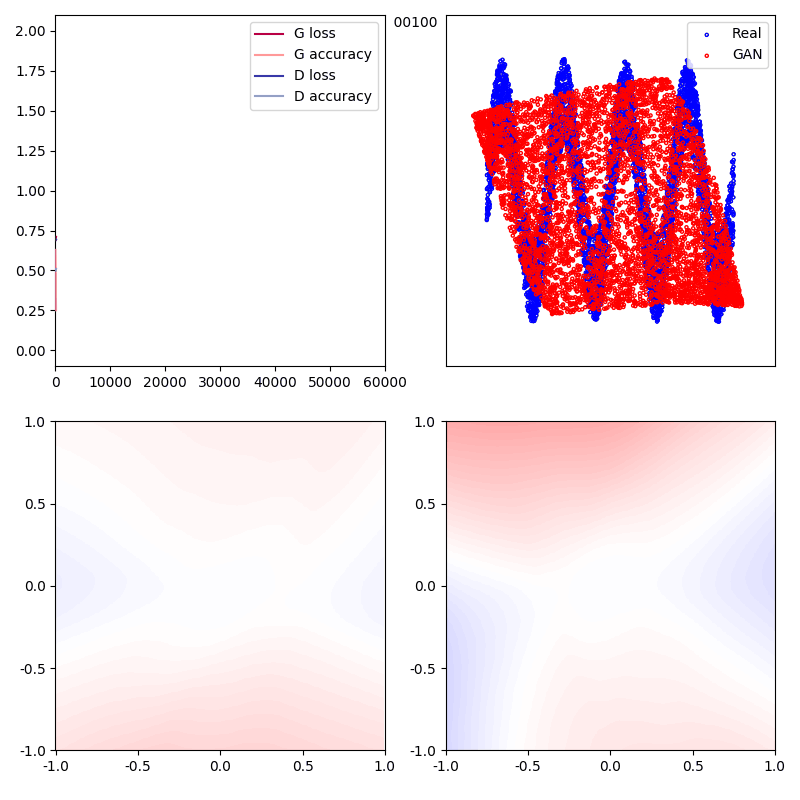
\includegraphics[width=0.75\textwidth]{sin_2_1}
  \caption{训练过程可视化的样图, 左上为损失函数, 右上为真实与伪造样本, 左下为输入的噪声空间的判别器输出, 右下为样本空间的判别器输出.}
\end{figure}

\begin{enumerate}
	\item 左上方可以看到每个训练步骤的生成器和判别器的损失(二进制交叉熵)和精度.
	\item 右上方为真实样本和伪造样本, 在每个训练步骤之后,绘制真实分布(蓝色)和生成的分布(红色).
	\item 左下方显示了隐空间中每个点的判别器输出,其中深蓝色表示判别器认为是“绝对是真的”,深红色表示判别器认为是“绝对是假的”,而白色表示判别器不知道该将其归为哪一类。
	\item 右下方图与左下方的图非常相似,不同之处在于它使样本空间而不是隐空间可视化了。
\end{enumerate}

\subsection{正弦波}

我们实验的第一个变换是将整个方块变换为正弦波, 即
\begin{align}
	f_x(x,y)&=x\\
	f_y(x,y)&=sin(x)+\dfrac{y}{4}
\end{align}

\begin{figure}[hbt]
\centering
  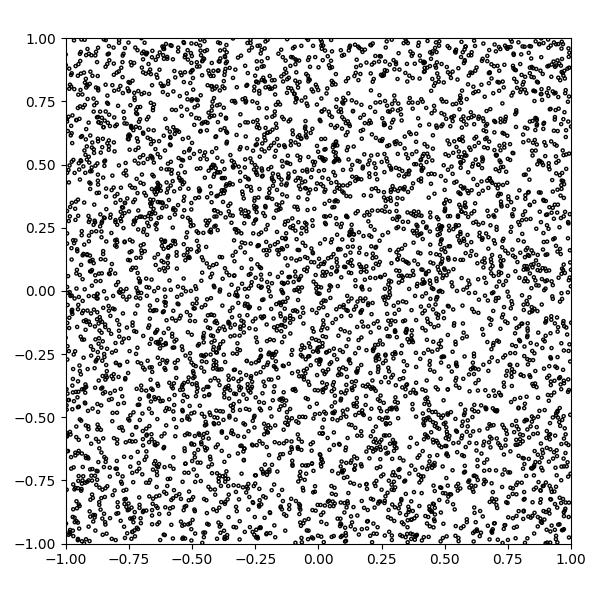
\includegraphics[width=0.23\textwidth]{sin_1_1}  
  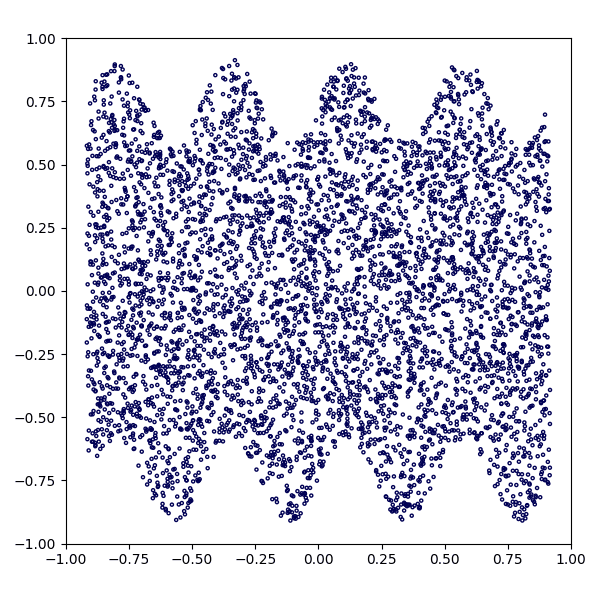
\includegraphics[width=0.23\textwidth]{sin_1_2}
  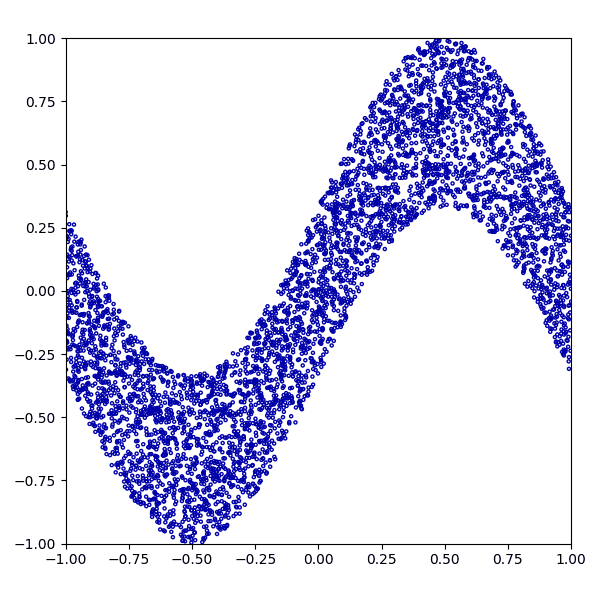
\includegraphics[width=0.23\textwidth]{sin_1_3}
  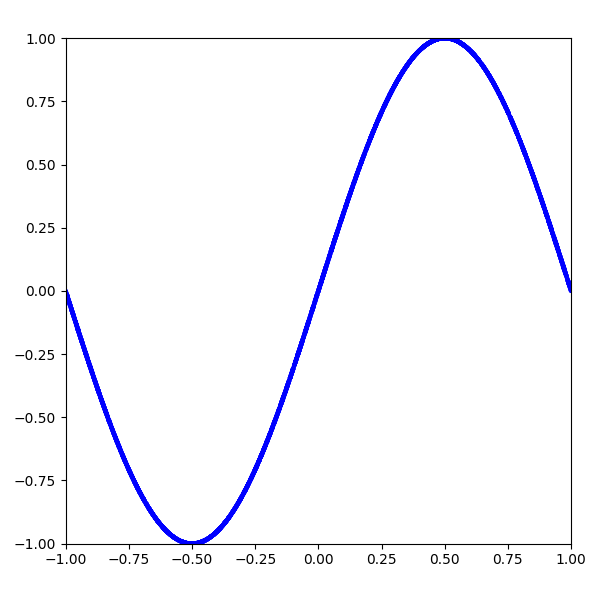
\includegraphics[width=0.23\textwidth]{sin_1_4}
  \caption{从左到右可以看出我们的变换$f$如何从Unif$[-1,1]^2$生成所需分布$\mathcal U$}
\end{figure}

我们得到的是一个在这个正弦波形区域里的均匀分布.

我们的实验发现这样的训练一共大概分三个时期. 捕捉大致范围, 捕捉细致分布到最后病态化.

\subsubsection{捕捉大致范围}

\begin{figure}[hbt]
\centering
  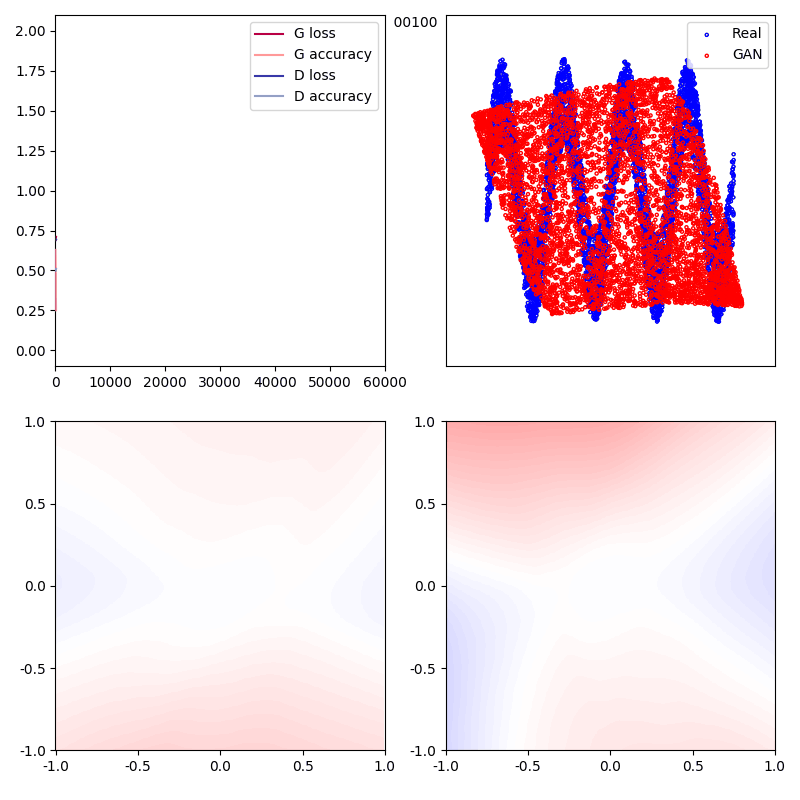
\includegraphics[width=0.45\textwidth]{sin_2_1}
  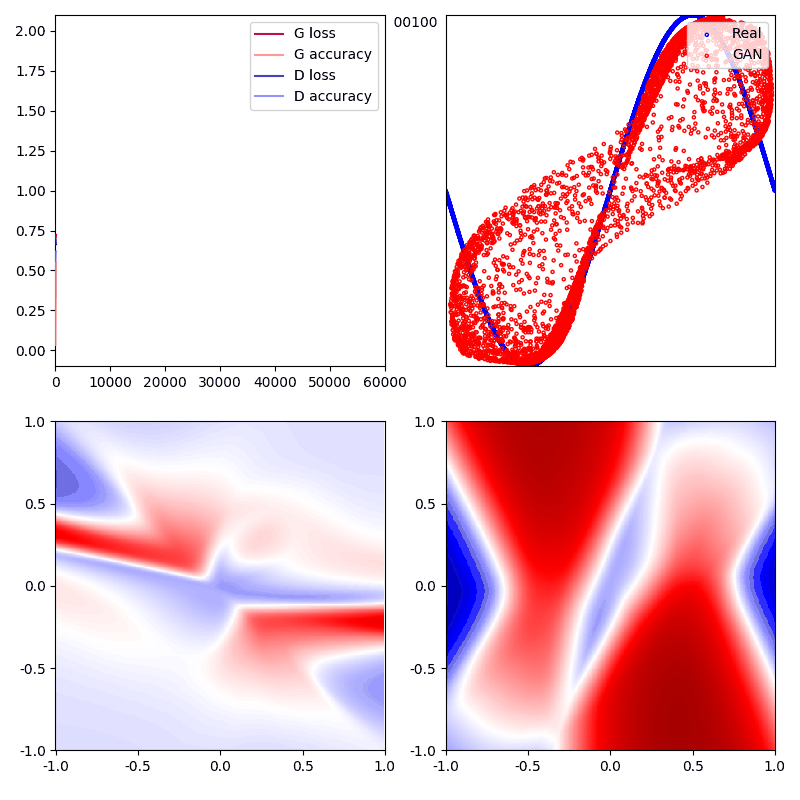
\includegraphics[width=0.45\textwidth]{sin_2_2}\\
  \caption{}
\end{figure}

首先我们看到在GAN得训练的初期阶段, 我们的分类器在帮助我们的生成器去捕捉一个大概的分布的范围. 并且很快我们的生成器就捕捉到了大致的范围, 可能是因为我们的函数比较简单.


\subsubsection{捕捉分布细节}

随着训练的进行, 我们发现一开始在捕捉到大致范围了以后, 生成器生成的点反而比较集中于两个波峰之间的白色区域里, 也就是没有生成出我们需要的样本. 但是慢慢的我们的辨别器成功地帮我们的生成器矫正了这些错误. 我们的生成器在经过15000次训练了以后表现已经不错了. 只有少部分点落在了白色区域, 大部分点都集中在了真实样本所在的区域. 这个时候我们的生成器已经可以代替我们的$f$来进行数据生成的工作了. 并且我们可以看到此时我们的分类器也大致出现了正弦波样式的分类边界, 这意味着我们得分类器应该是要继续执导我们的生成器使得生成器在白色区域的生成样本逐渐越来越少. 但是事情并不是这样发展的.

\begin{figure}[hbt]
\centering
  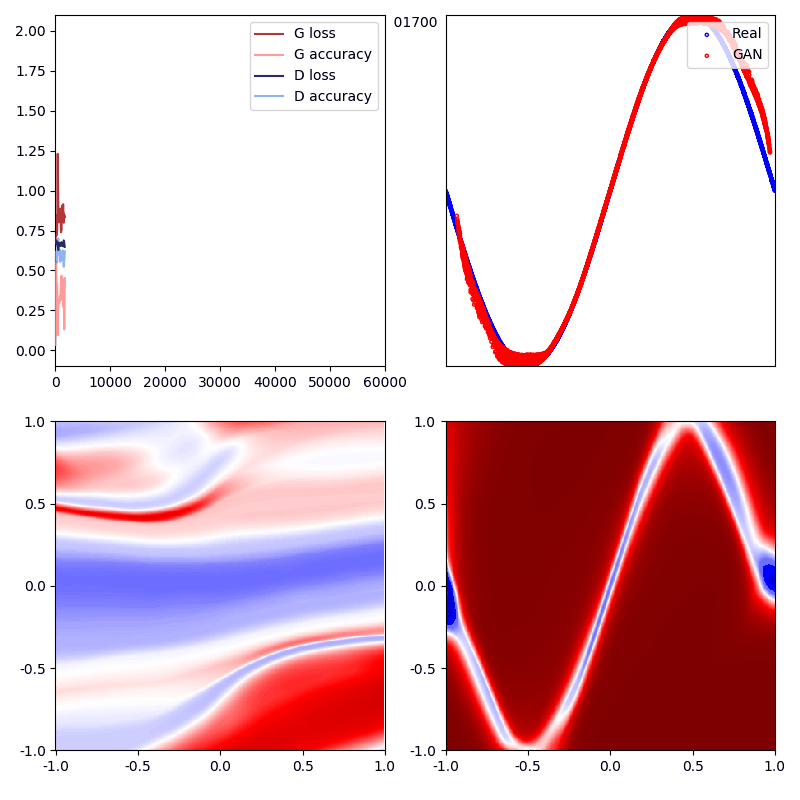
\includegraphics[width=0.45\textwidth]{sin_3_1}
  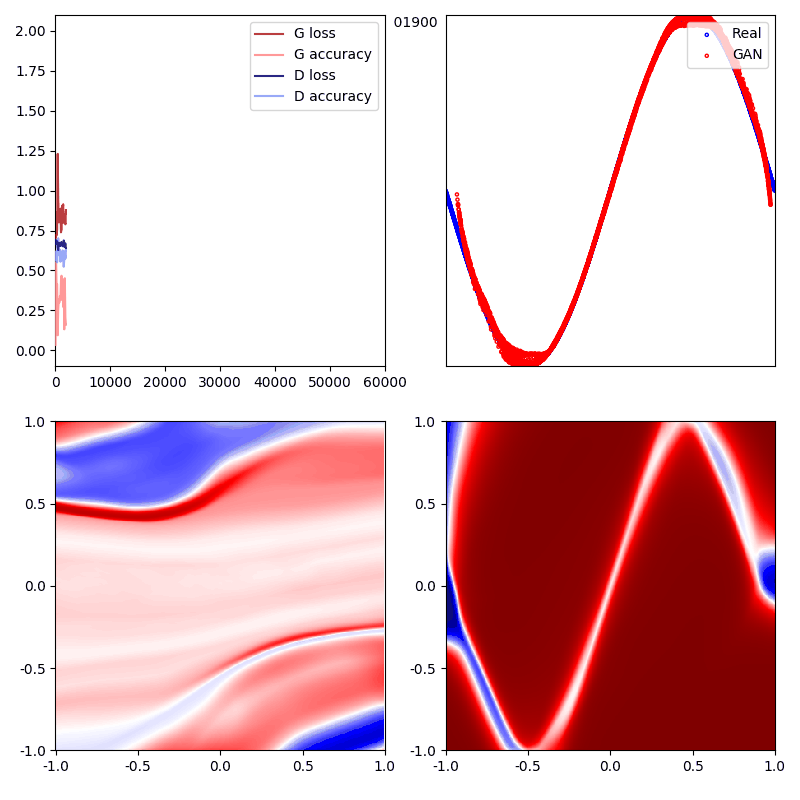
\includegraphics[width=0.45\textwidth]{sin_3_2}\\
  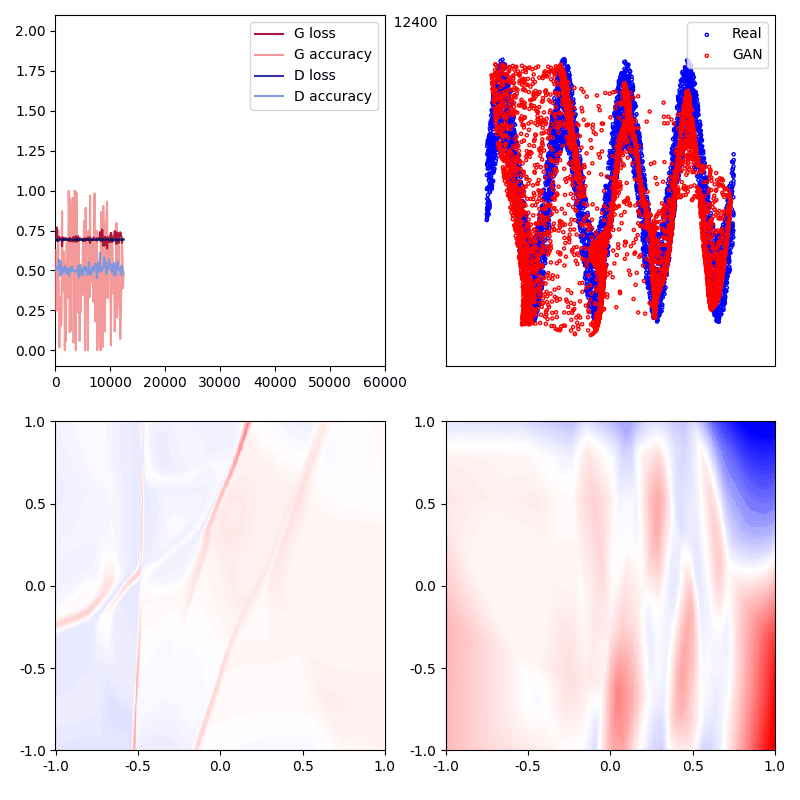
\includegraphics[width=0.45\textwidth]{sin_3_3}
  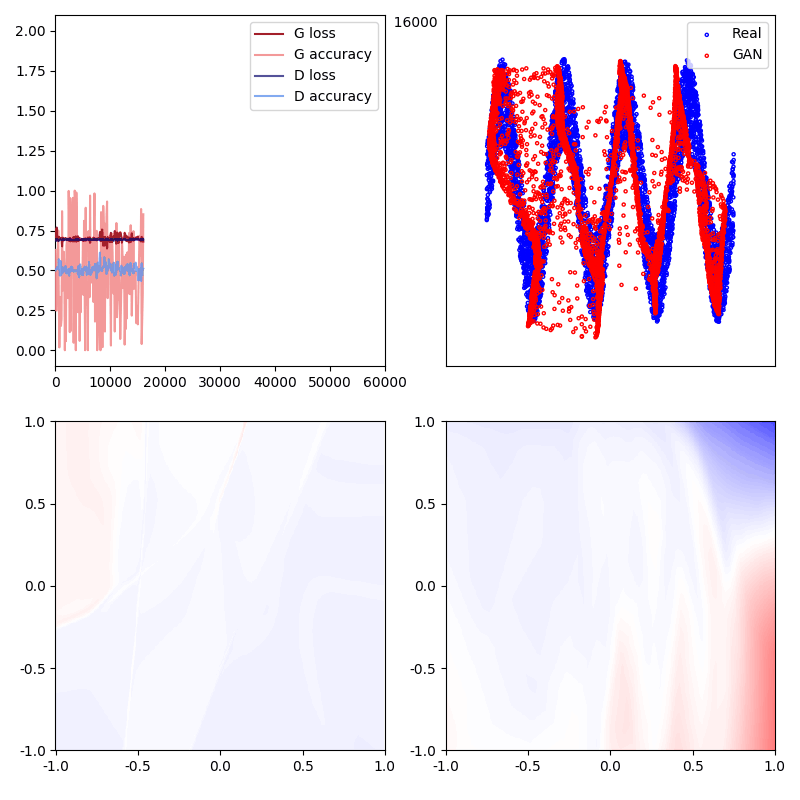
\includegraphics[width=0.45\textwidth]{sin_3_4}
  \caption{}
\end{figure}

%并且随着训练的进行, 我们的辨别器捕捉到的在样本空间中的分类边界反而变得比一开始更加模糊, 之前认为是真实样本的区域完全消失掉了. 原来样本空间中正弦波样式的分类边界逐渐消失变为了一整个辨别器无法确定真假的长方形区域. 并且我们在输入空间中的辨别器输出大部分都变为了不确定. 同时生成器也出现了较大的波动. 

\subsubsection{病态化}

随着训练的继续, 我们发现我们的GAN陷入了一个无法跳出的怪圈. 我们的分类器指导我们的生成器向着一个错误的方向进行了改进, 并且自从陷入进去以后, 一直到60000次训练结束的时候我们还是看不到任何的改善. 首先我们的在白色区域的生成样本逐渐变多. 逐渐回到了刚刚捕捉到大范围时的状态. 并且可以很明显的看到我们的生成器还因为未知的原因在一条对角线上集中地在生成数据, 我们怀疑我们的训练陷入了一个局部极小值的状态. 此时我们的辨别器对我们的生成器没有办法进行有效的指导. 我们认为这样的现象有如下几种可能

\begin{enumerate}
	\item 网络太浅, 表达能力不足.
	\item 训练次数不够.
	\item 超参不合适.
\end{enumerate}

我们通过进一步的实验的现象猜测最有可能是因为超参数的设置不合理. 进一步实验的细节见后.

\begin{figure}[hbt]
  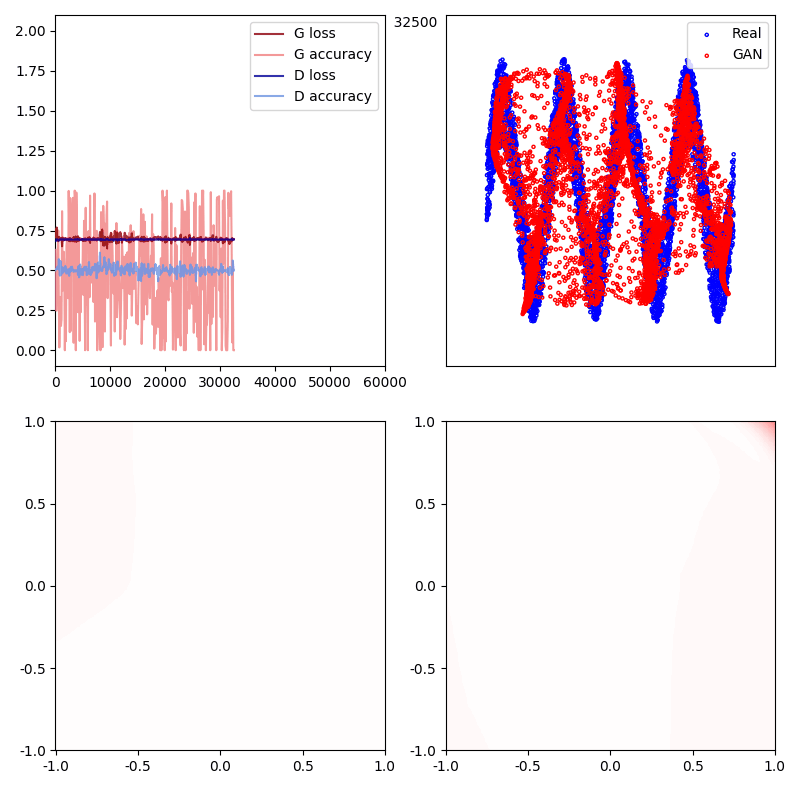
\includegraphics[width=0.3\textwidth]{sin_4_1}
  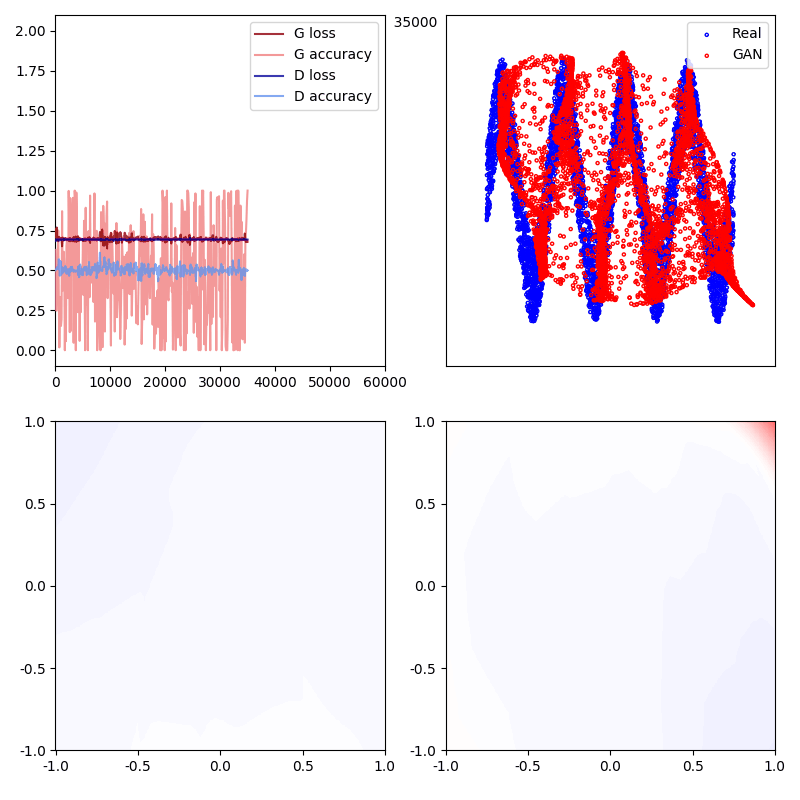
\includegraphics[width=0.3\textwidth]{sin_4_2}
  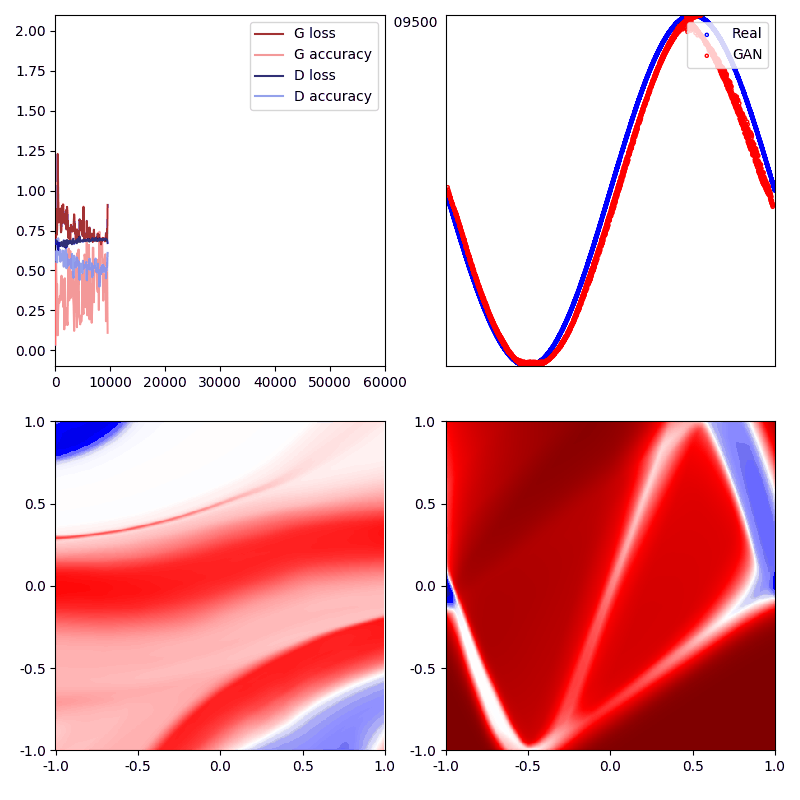
\includegraphics[width=0.3\textwidth]{sin_4_3}\\
  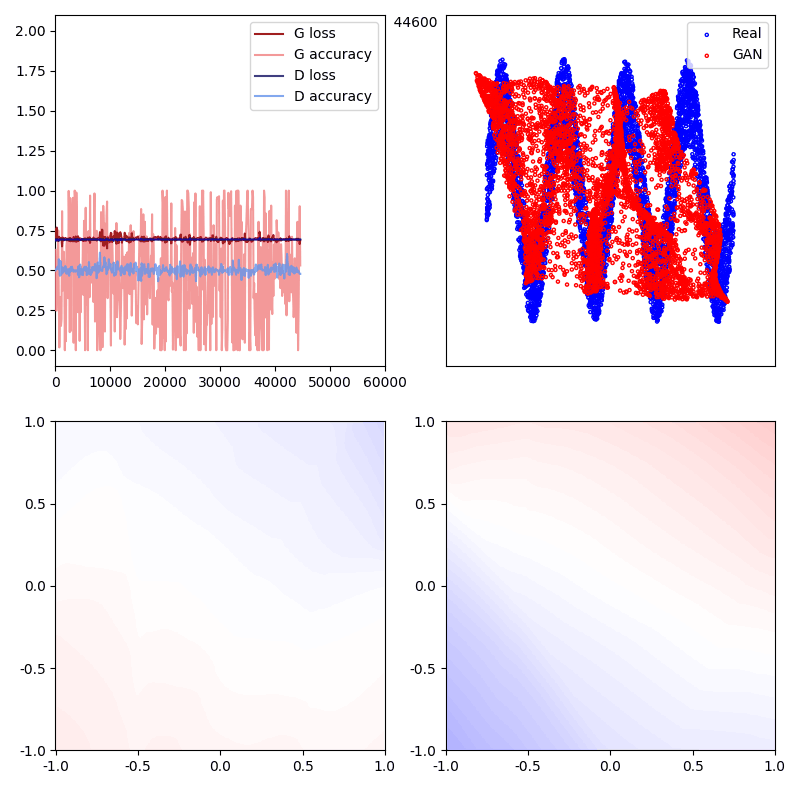
\includegraphics[width=0.3\textwidth]{sin_4_4}
  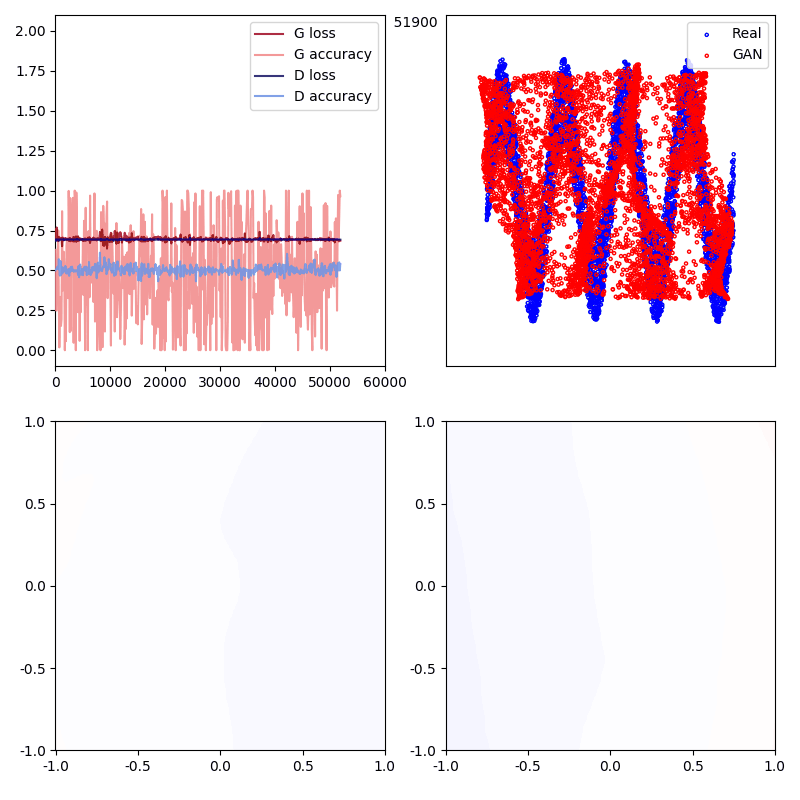
\includegraphics[width=0.3\textwidth]{sin_4_5}
  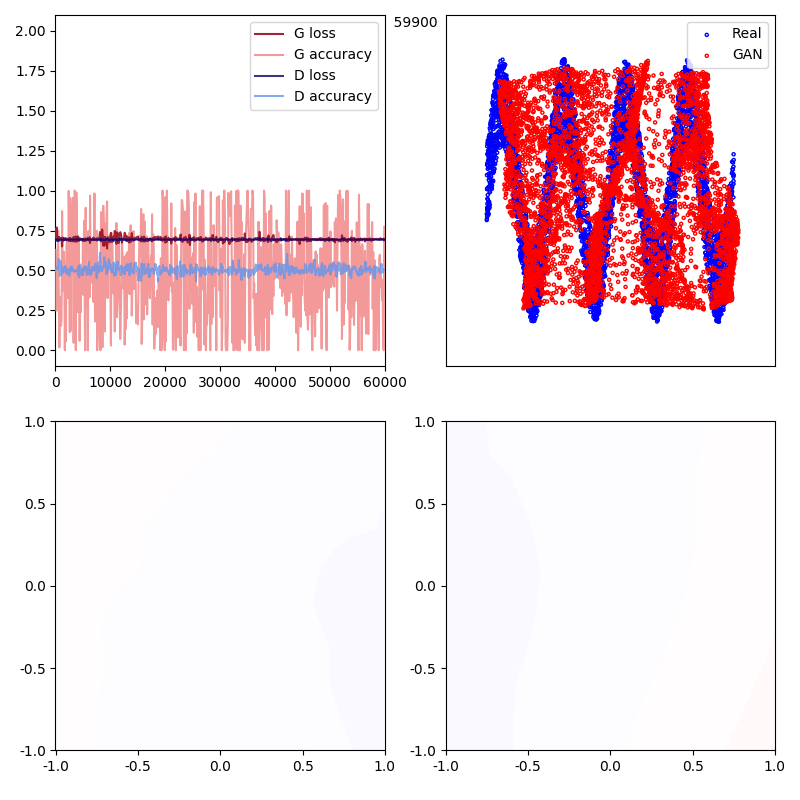
\includegraphics[width=0.3\textwidth]{sin_4_6}
  \caption{}
\end{figure}


\subsection{圆}

我们实验的第二个变换是将整个方块变为一个半径为1的圆, 即
\begin{align}
	f_x(x,y)&=x/2 \\
	f_y(x,y)&=y\pi
\end{align}

\begin{figure}[hbt]
\centering
  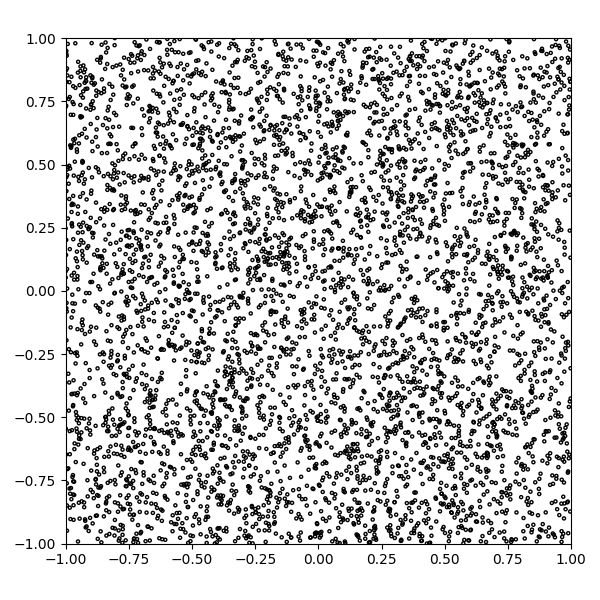
\includegraphics[width=0.23\textwidth]{circle_1_1}
  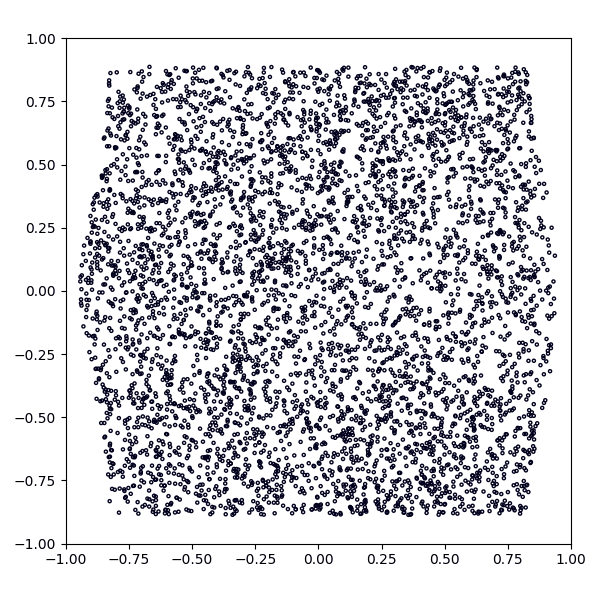
\includegraphics[width=0.23\textwidth]{circle_1_2}
  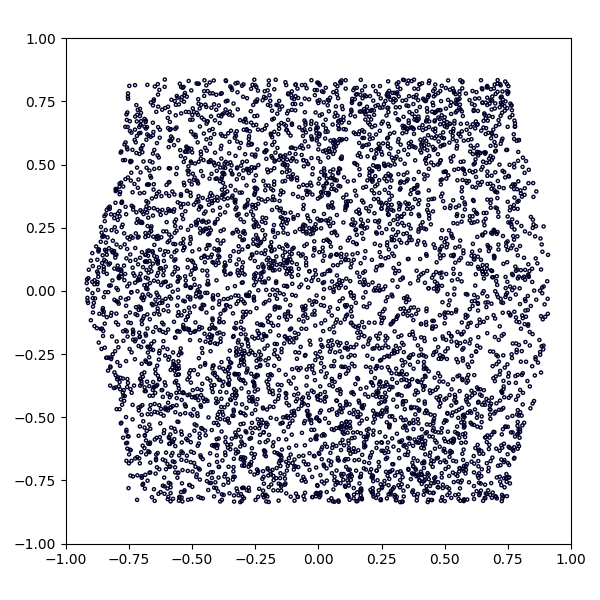
\includegraphics[width=0.23\textwidth]{circle_1_3}
  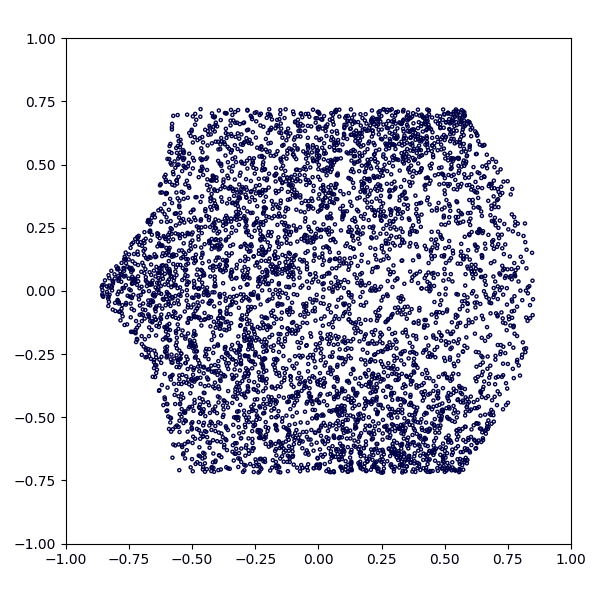
\includegraphics[width=0.23\textwidth]{circle_1_4}\\
  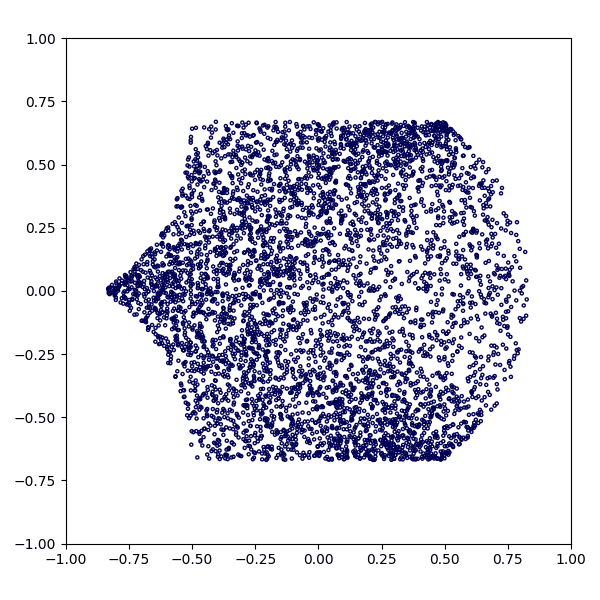
\includegraphics[width=0.23\textwidth]{circle_1_5}
  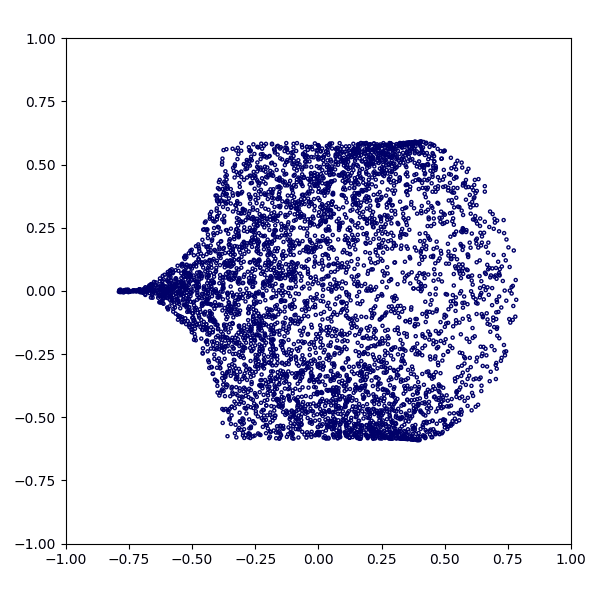
\includegraphics[width=0.23\textwidth]{circle_1_6}
  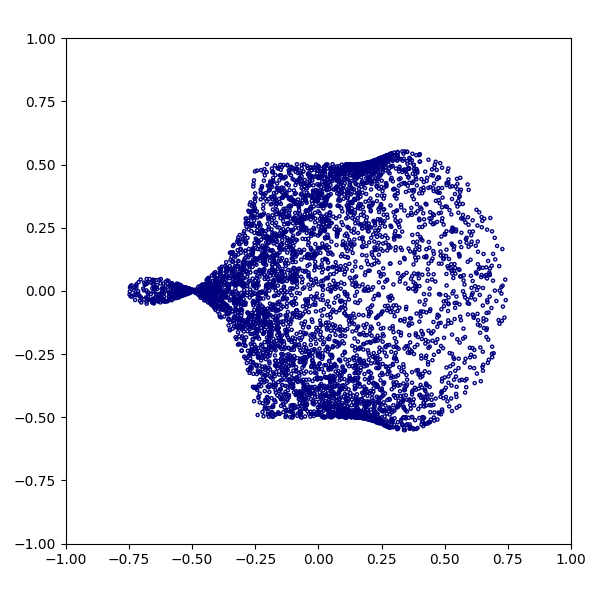
\includegraphics[width=0.23\textwidth]{circle_1_7}
  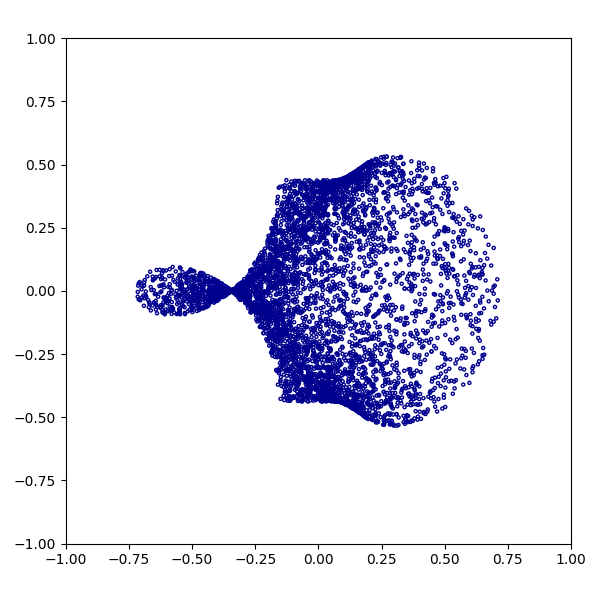
\includegraphics[width=0.23\textwidth]{circle_1_71}\\
  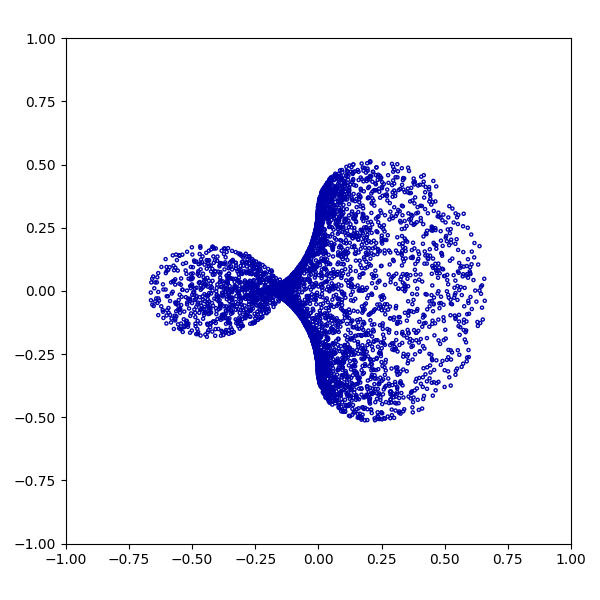
\includegraphics[width=0.23\textwidth]{circle_1_8}
  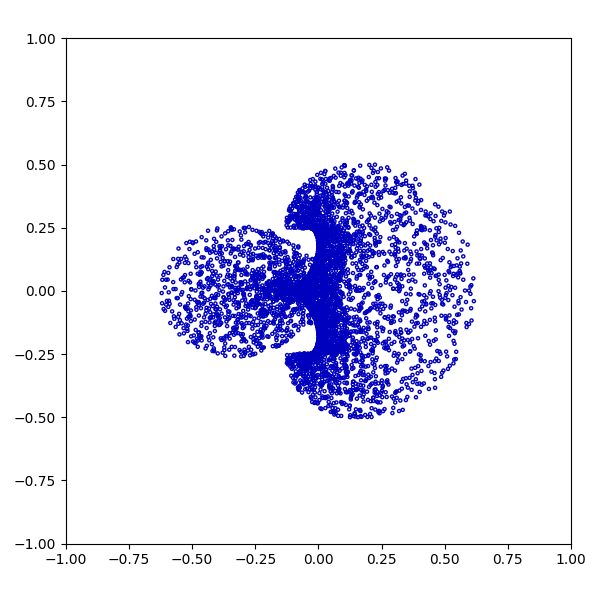
\includegraphics[width=0.23\textwidth]{circle_1_81}
  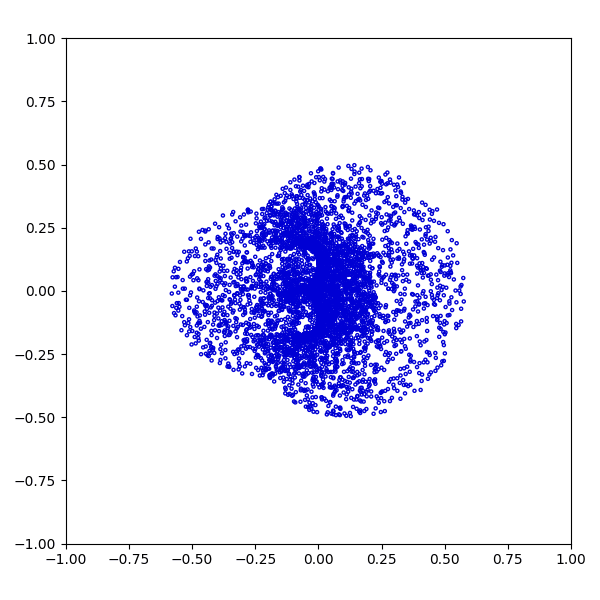
\includegraphics[width=0.23\textwidth]{circle_1_9}
  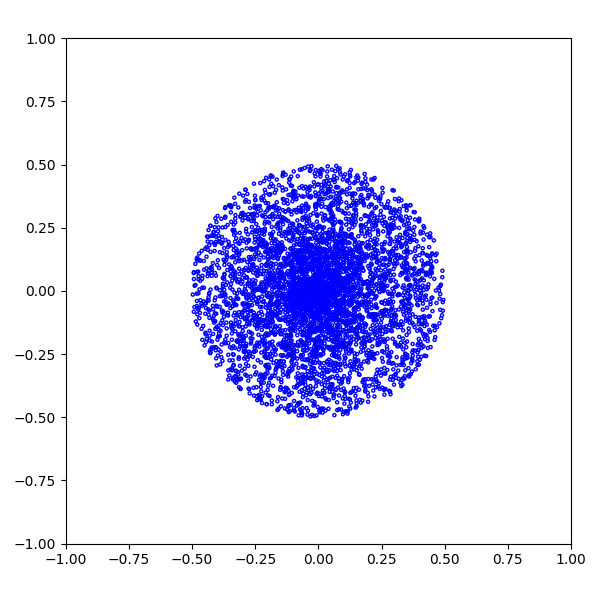
\includegraphics[width=0.23\textwidth]{circle_1_10}  
  
  \caption{从左上到右下可以看出我们的变换$f$如何从Unif$[-1,1]^2$生成所需分布$\mathcal U$}
\end{figure}



我们可以证明这样变换得到的分布并不是在这个圆上的一个均匀分布. 从图上也可以看出这样的分布下, 数据更有可能处于中心而不是圆的边缘.

\begin{figure}[hbt]
  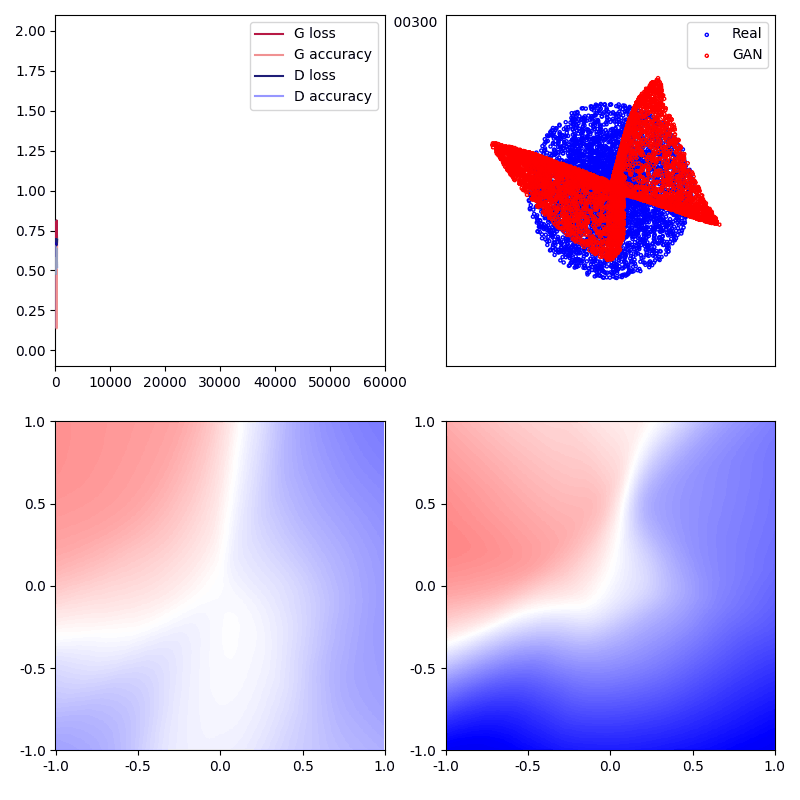
\includegraphics[width=0.45\textwidth]{circle_2_1}
  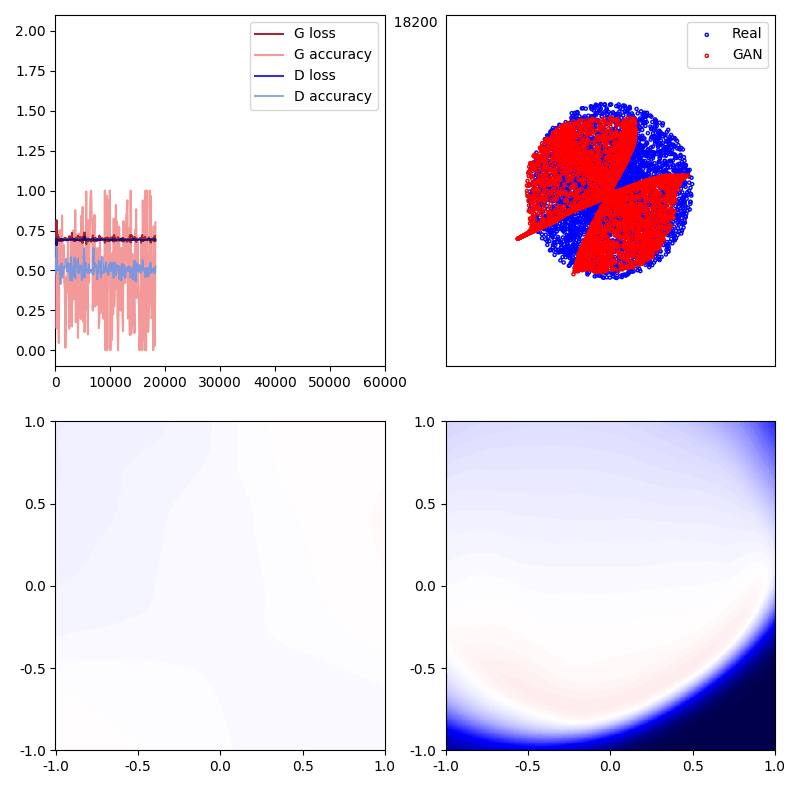
\includegraphics[width=0.45\textwidth]{circle_2_2}\\
  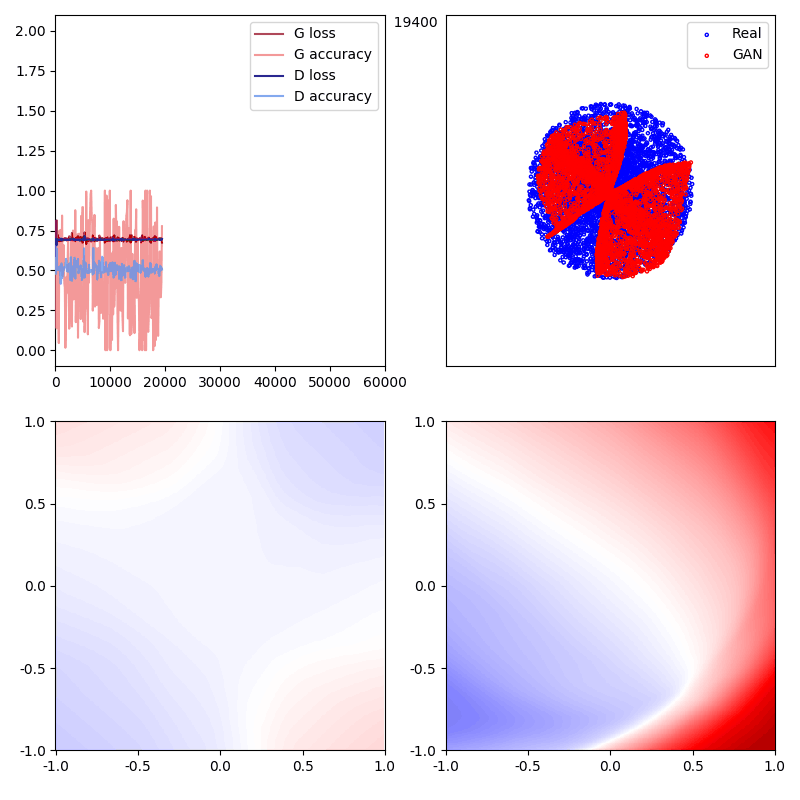
\includegraphics[width=0.45\textwidth]{circle_2_3}
  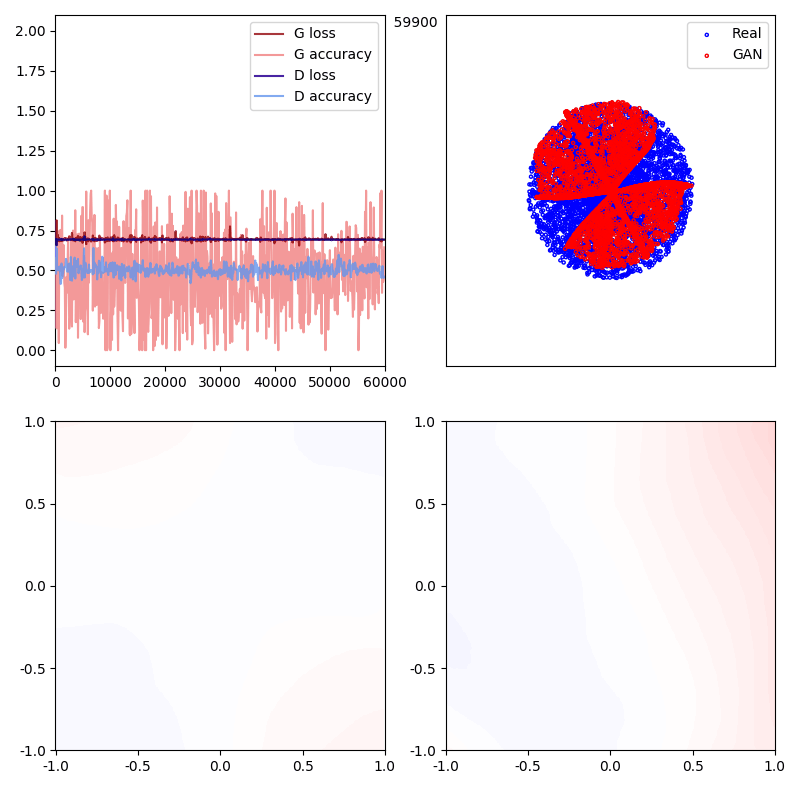
\includegraphics[width=0.45\textwidth]{circle_2_4}
  \caption{我们可以看到我们的生成器生成的样本并非如我们所想的是圆形, 反而是一个蝴蝶型. 并且我们之前观察到的辨别器的输出翻转在右上与左下之间也观察到了混沌的现象, 其仅相隔一个batch辨别器却给出了完全推翻之前结论的结果.}
\end{figure}

我们可以看到我们的生成器并没有像我们想象一样捕捉到圆形分布. 但是它捕捉到了分布的大致范围, 以及分布密度从中间到外围逐渐递减的特点. 其生成的样本因为某种未知的原因呈一个蝴蝶型. 并且其捕捉到这个蝴蝶型的分布十分迅速, 在训练的过程中一直保持着这样的蝴蝶型. 同时在训练结束的时候我们的辨别器基本上处于躺平的状态, 对所有的样本都无法给出有效的判断, 自然也无法对生成器进行有效的有意义的引导. 我们还注意到在训练的过程中, 我们的判别器的行为有着一定的混沌性. 很多次只间隔一个batch就完全地推翻了之前所给出的结果, 图上的表现就是前一个batch里红色与蓝色的分布的地方在一个batch的训练后发生了彻底的翻转.



\subsection{翅膀型}

我们最后一个实验的变换是一个翅膀型(两个螺线拼接), 即
\begin{align}
	f_x(x,y) &= \dfrac{x}{2} \cos (3x\pi) \\
	f_y(x,y) &= \dfrac{x}{2} \sin (3x\pi)
\end{align}

\begin{figure}[hbt]
\centering
  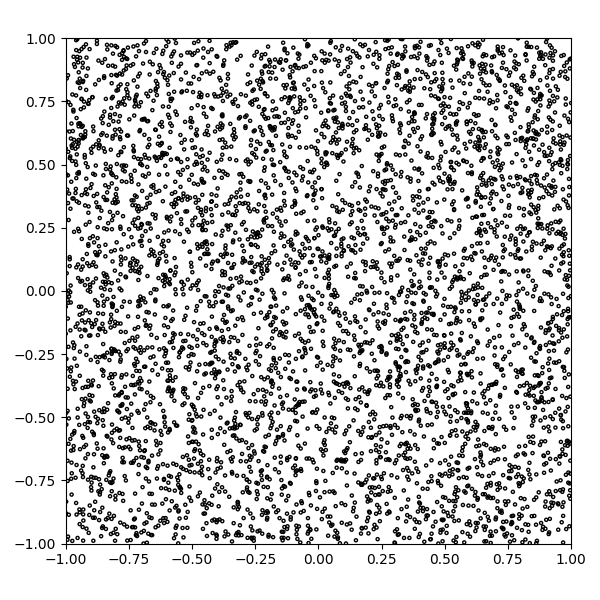
\includegraphics[width=0.23\textwidth]{wings_1_1}
  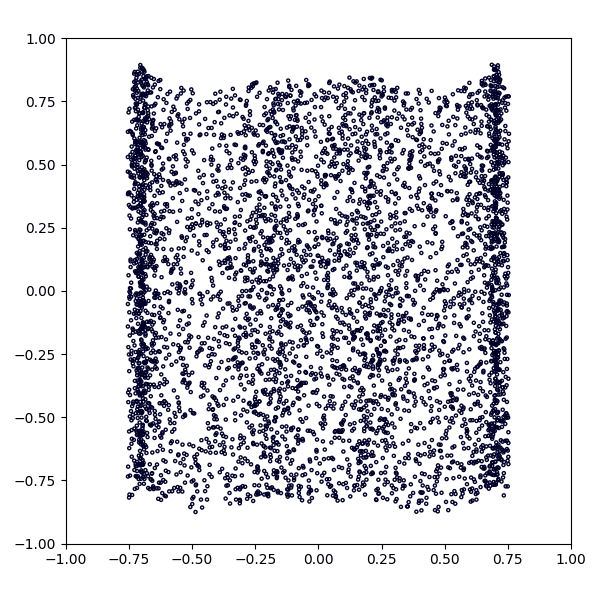
\includegraphics[width=0.23\textwidth]{wings_1_2}
  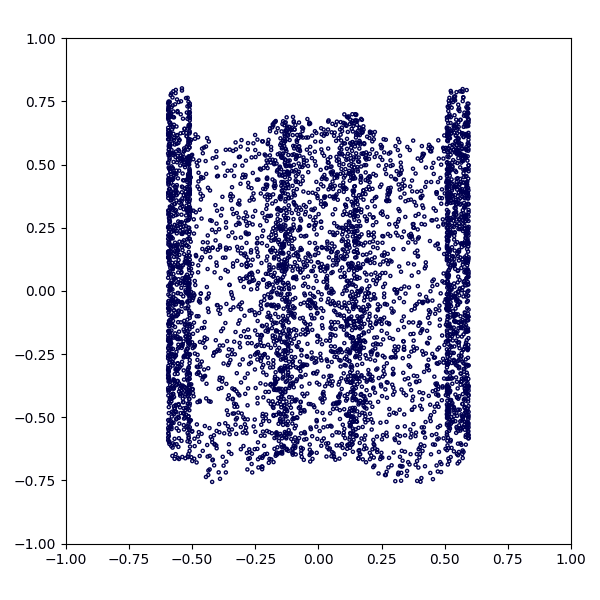
\includegraphics[width=0.23\textwidth]{wings_1_3}
  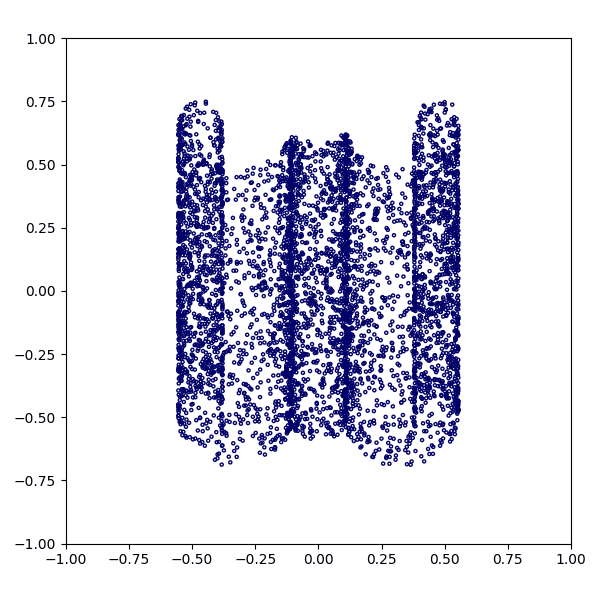
\includegraphics[width=0.23\textwidth]{wings_1_4}\\
  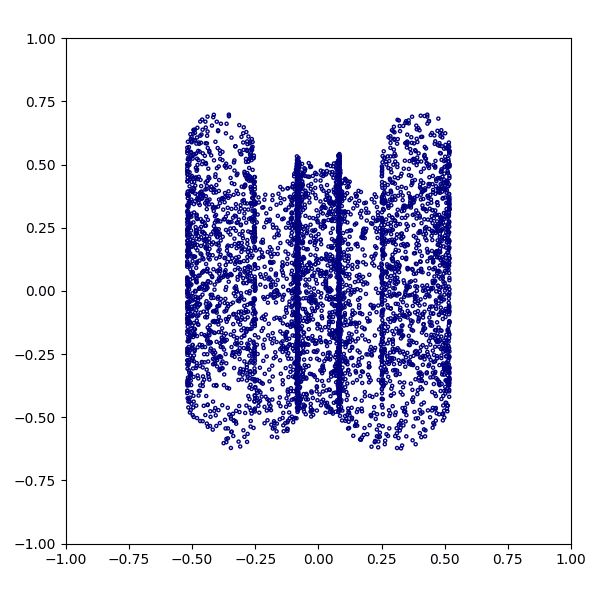
\includegraphics[width=0.23\textwidth]{wings_1_5}
  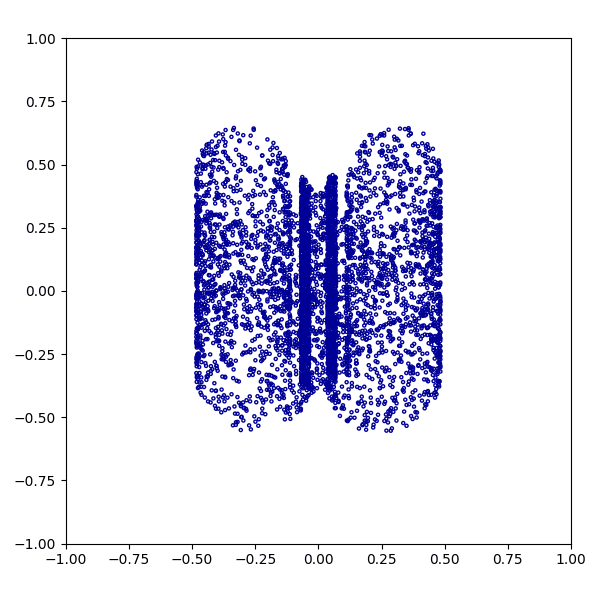
\includegraphics[width=0.23\textwidth]{wings_1_6}
  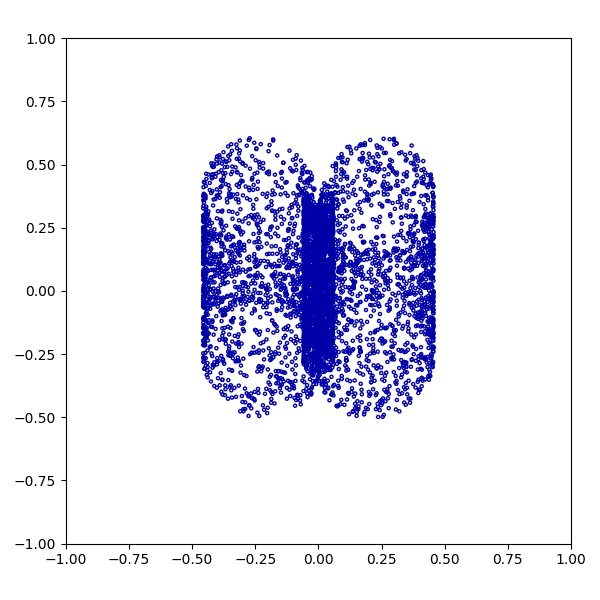
\includegraphics[width=0.23\textwidth]{wings_1_7}
  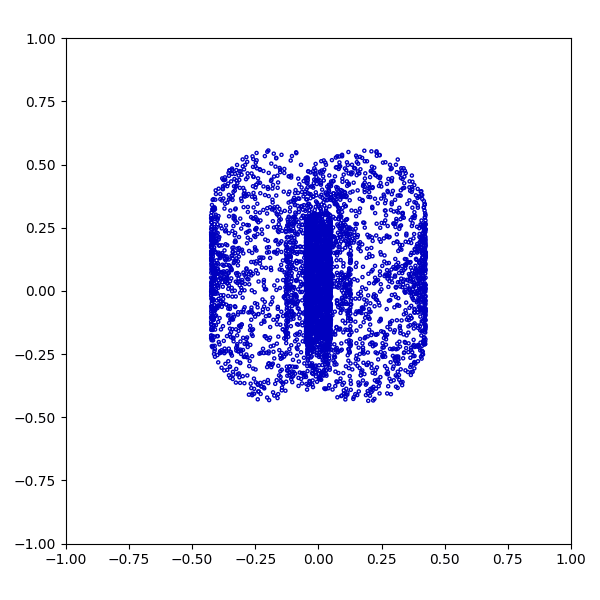
\includegraphics[width=0.23\textwidth]{wings_1_8}\\
  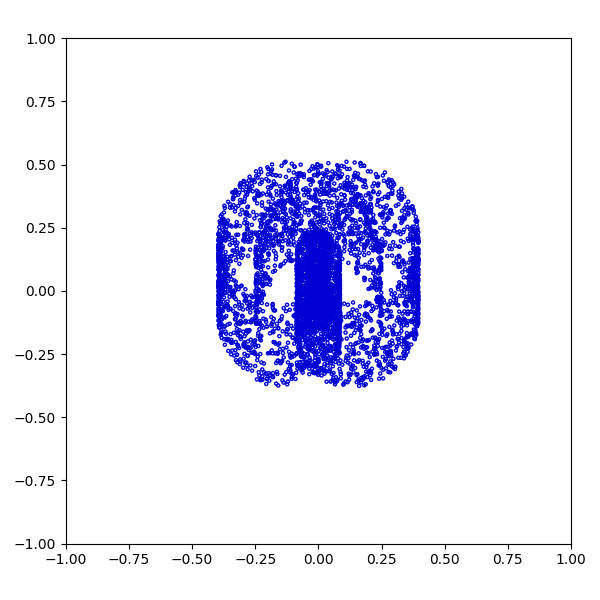
\includegraphics[width=0.23\textwidth]{wings_1_9}
  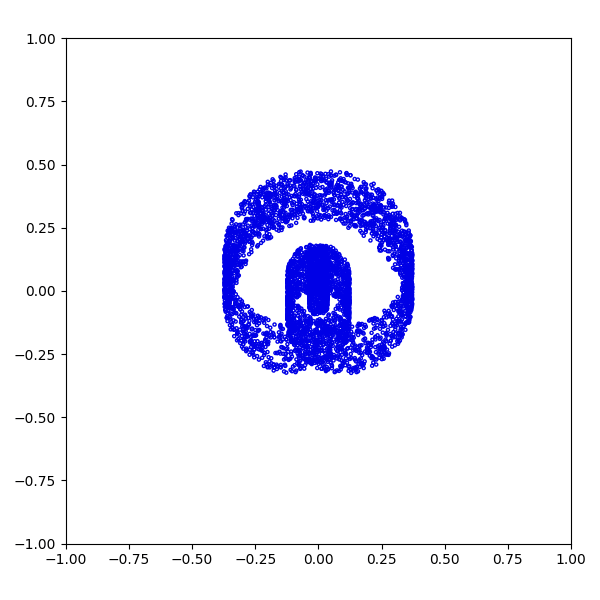
\includegraphics[width=0.23\textwidth]{wings_1_10}
  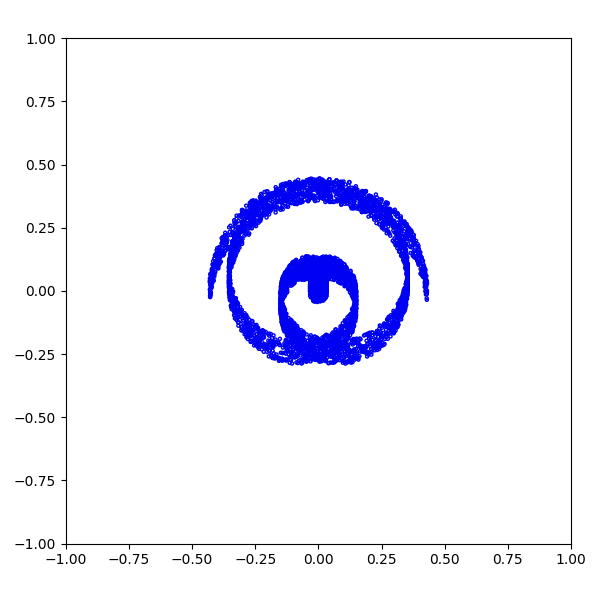
\includegraphics[width=0.23\textwidth]{wings_1_11}
  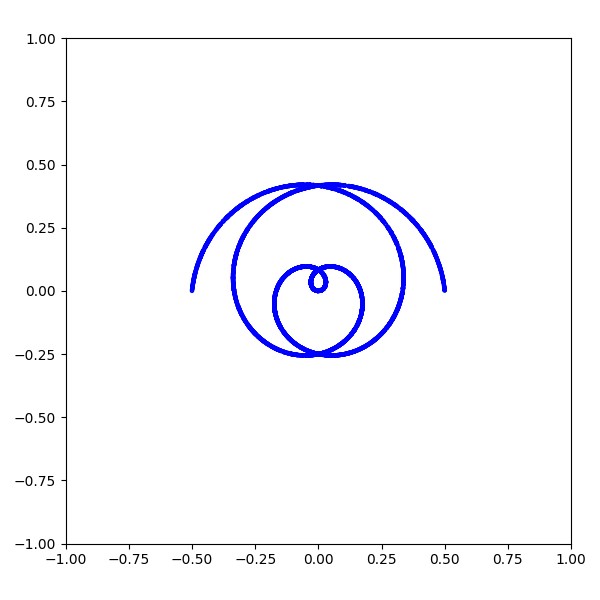
\includegraphics[width=0.23\textwidth]{wings_1_12}

  
  \caption{从左上到右下可以看出我们的变换$f$如何从Unif$[-1,1]^2$生成所需分布$\mathcal U$}
\end{figure}

这个分布在他的支集上也并非一个均匀分布, 我们通过变换的过程的可视化以及理论证明都可以得到相同的结果.

\subsubsection{捕捉大致范围}

\begin{figure}[hbt]
\centering
  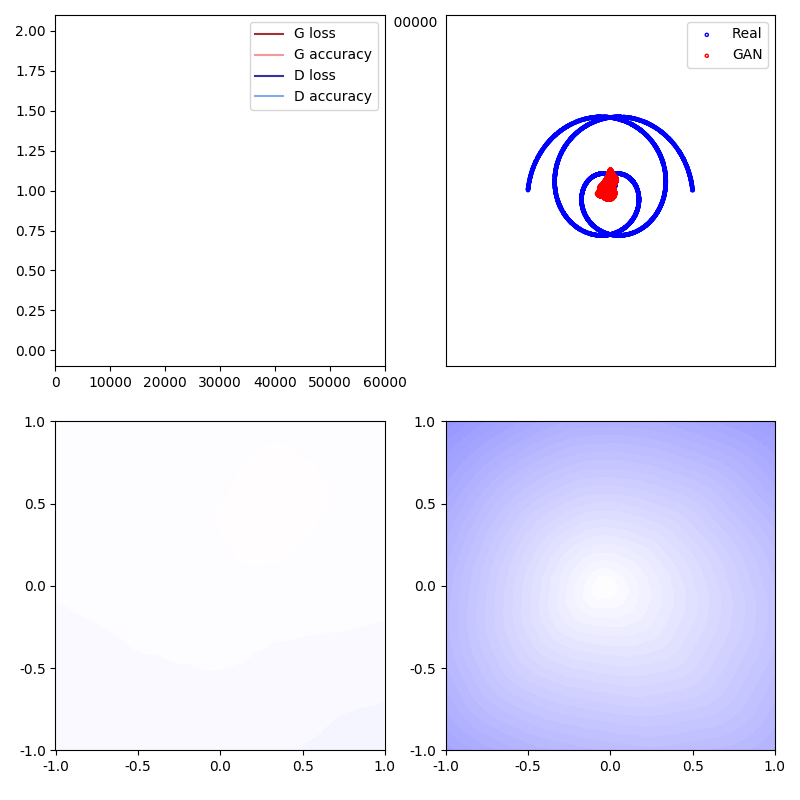
\includegraphics[width=0.45\textwidth]{wings_2_1}
  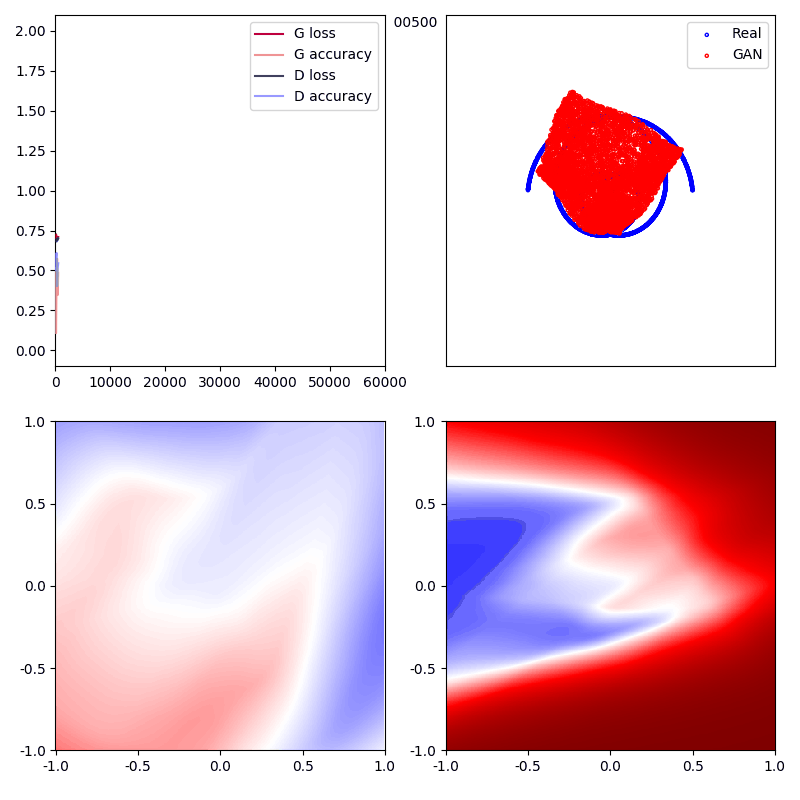
\includegraphics[width=0.45\textwidth]{wings_2_2}\\
  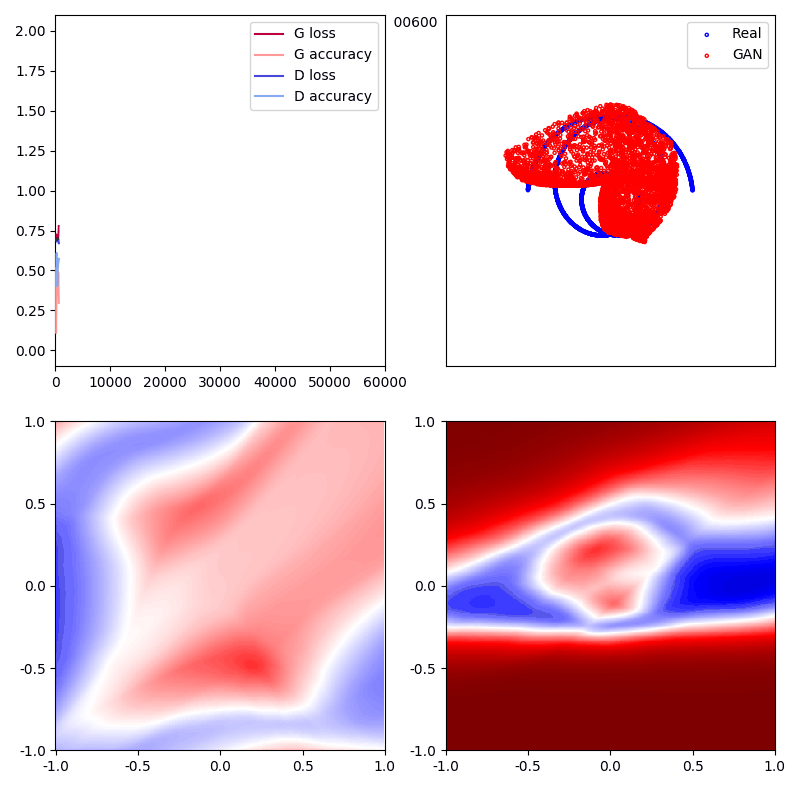
\includegraphics[width=0.45\textwidth]{wings_2_3}
  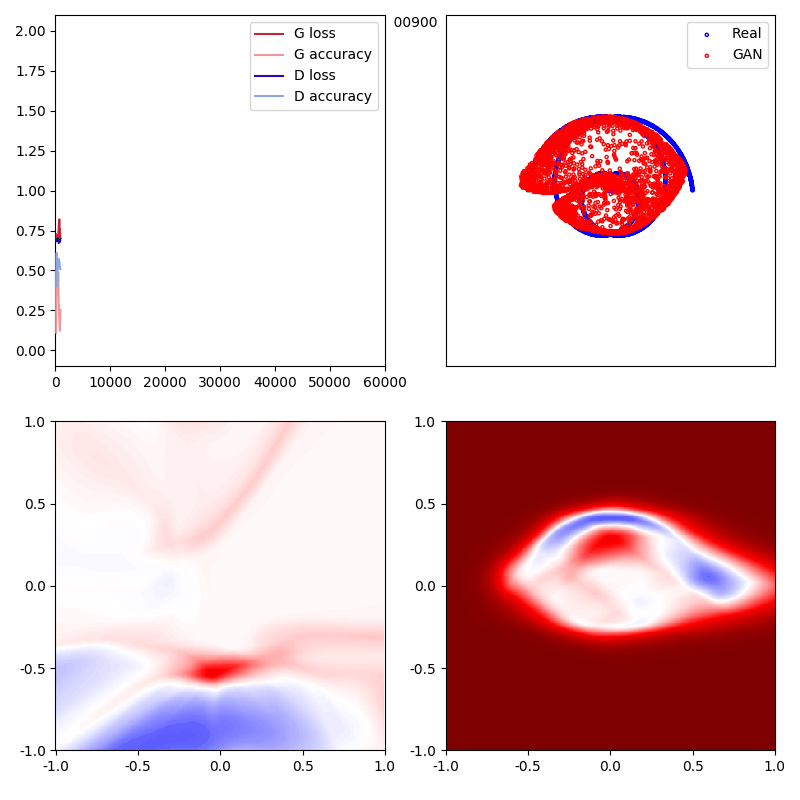
\includegraphics[width=0.45\textwidth]{wings_2_4}
  \caption{我们可以看到生成器与辨别器在训练开始先去捕捉了真实样本所处的大致范围, 并且在输入空间的中下部中逐渐出现了一个深红色块(代表着辨别器以很高的置信度将这一片区域判别位了生成样本), 我们可以猜测此时生成器将这部分映射到了样本空间的边角}
\end{figure}

我们可以看到这次生成器首先去捕捉了大概的样本所处的范围. 同时辨别器也在捕捉真实样本所处的大范围. 并且在输入空间的中下部出现了一个置信度极高的假样本区域(深红色区域), 我们猜测我们的生成器将这部分区域映射到了样本空间的外侧边角.

\subsubsection{捕捉分布细节}

\begin{figure}[hbt]
  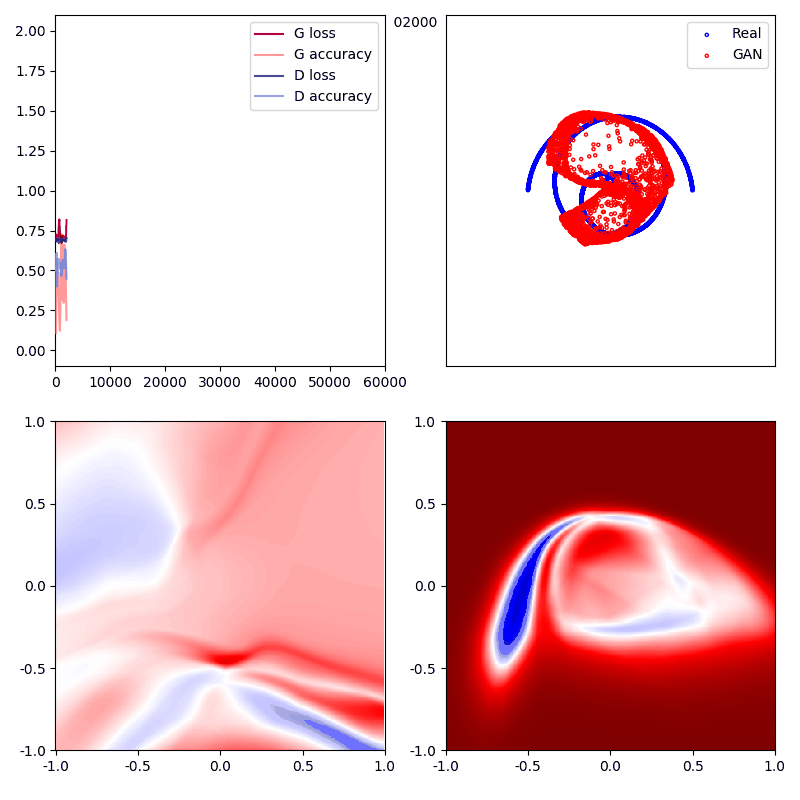
\includegraphics[width=0.33\textwidth]{wings_3_1}
  \includegraphics[width=0.33\textwidth]{wings_3_2}
  \includegraphics[width=0.33\textwidth]{wings_3_3}\\
  \includegraphics[width=0.33\textwidth]{wings_3_4}
  \includegraphics[width=0.33\textwidth]{wings_3_5}
  \includegraphics[width=0.33\textwidth]{wings_3_6}\\
  \includegraphics[width=0.33\textwidth]{wings_3_7}
  \includegraphics[width=0.33\textwidth]{wings_3_8}
  \caption{我们可以看到在样本空间中逐渐出现了一个高置信的真实样本区域(深蓝色), 这个区域随着训练的进行从左下角出现然后逐渐延伸到两侧, 再逐渐收小最后达到最终结果. 同时随着这个蓝色区域的出现与收缩, 我们的生成器并没有在这两个蓝色区域相应的位置生成样本.}
\end{figure}

我们可以看到随着训练的进行, 我们的生成器逐渐捕捉到了分布集中在曲线上这一特点. 并且逐渐有更多的点附着到了曲线上. 而分类器这次的表现十分稳固, 在圆内的部分, 真实数据分布在一条曲线上的特征分类器也很好地捕捉到了. 有趣的是观察我们的分类器如何随着我们的生成器捕捉到分类边界. 首先一个高置信度的真实样本区间出现在左下角, 随着训练的进行逐渐右下角也出现了这样的一个真实样本区域, 然后两个区域逐渐分离并向上运动, 最后收缩成为两个翅膀的样子. 与此同时我们的生成器在一开始在两个翅膀的位置还是有生成样本的, 但是随着这两个高置信度真实样本区间的出现与收紧, 他就再也没有生成出任何在这两个翅膀的区域上的样本了. 可以说我们的GAN在这个圆里达到了平衡, 但是在翅膀的部分我们的辨别器完全主宰了我们的生成器. 

同时我们这个时候我们再看之前观测到的那个红色区域, 我们可以发现这个红色区域在此时变成了红色与蓝色交叉的区域, 同时样本空间中的边缘也是红色蓝色相间的. 我们基本上可以断定我们的生成器把这个部分映射到了样本空间的边角上.

\section{超参对比}

我们实验了多组网络的学习率与Adam的参数, 对前面研究过的三个模型再进行了实验. 其中圆的训练结果没有任何的改变, 然而正弦波与翅膀型我们通过观察其在不同参数下的表现发现了一些比较有趣的结果. 我们挑选了两组我们认为最能说明问题的参数来进行展示.

\subsection{正弦波}

我们将生成器与分类器的优化算法adam的参数$\beta$从0.5改到了0.7. 我们可以看到我们的网络依旧能够捕捉到我们的大致分布的范围. 但是却无法捕捉到任何细致的分布. 同时我们还能够观察到在前面实验里出现的样本集中到对角线上的情况迅速的出现. 并且在这个现象出现以后, 我们的网络便几乎停止了更新. 尽管我们可以明显地看到大部分样本反而集中在两个波峰之间的空白区域, 但是我们的辨别器已经无法指导我们的分类器进行更新了. 所以我们猜测我们之前所观察到的现象是陷入到了一个局部极小值中. 我们的网络在陷入了以后无法自己通过更新参数逃出这个陷阱.

\begin{figure}[hbt]
\centering
  \includegraphics[width=0.45\textwidth]{sin_6_1}
  \includegraphics[width=0.45\textwidth]{sin_6_2}\\
  \includegraphics[width=0.45\textwidth]{sin_6_3}
  \includegraphics[width=0.45\textwidth]{sin_6_4}
  \caption{}
\end{figure}



\subsection{翅膀型}

我们选择了一组新的参数, 生成器的学习率为0.0005, Adam参数为$\beta=0.9$. 分类器的学习率为0.05, Adam参数为$\beta=0.9$. 我们发现在这样的参数设定下, 我们的生成器甚至无法捕捉到初始的分布的轮廓. 其生成的数据缩小成了一小块区域, 围绕真实数据进行震荡, 随着训练的进行这样的震荡更多地集中在了数据中心.

\begin{figure}[hbt]
\centering
  \includegraphics[width=0.45\textwidth]{wings_4_1}
  \includegraphics[width=0.45\textwidth]{wings_4_2}\\
  \includegraphics[width=0.45\textwidth]{wings_4_3}
  \includegraphics[width=0.45\textwidth]{wings_4_4}
  \caption{}
\end{figure}



\nocite{*}

% 如果想修改参考文献样式(非国标),请把下行取消注释,并换成合适的样式(比如 unsrt,plain 样式)。
\bibliographystyle{unsrt}
\bibliography{wpref}

\end{document}
